\section{Multiplicity-sensitive upper-bound arguments}
\label{upper:scope}

This section develops restricted upper estimates by separating the ordinary part of an arrangement from its finite multiple points. The geometric derivations below are ordinary mathematical proofs. The local fan geometry and cyclic counting are formalized in Lean, while the extraction of elementary segments from an arbitrary arrangement and the global clean-line charging argument are not. Accordingly, this section does not assert a completed Lean upper theorem for all arrangements, and none of its restricted conclusions is an improved upper bound for the full function $\K$.

The distinction is necessary because the even-order estimates of Bartholdi--Blanc--Loisel and Blanc require simplicity~\citep{bbl2008,blanc2011}. The classical Cl\'ement--Bader envelope is treated as a reported external theorem~\citep{clementbader2007}; the local example in Section~\ref{upper:shared-fan} explains why we do not silently replace its proof by a bound on all shared edges incident to a multiple point.

\subsection{An exact elementary-segment identity}

\begin{definition}
For an arrangement of $n$ distinct affine lines, let $t_r$ be the number of finite intersection points incident to exactly $r$ lines, and let $P$ be the number of unordered parallel pairs. A bounded \emph{elementary segment} is the portion of an arrangement line between two consecutive finite intersection points. Let $E$ count these segments, $U$ count those incident to no triangular cell, and $D$ count those incident to two triangular cells. Let $a$ be the number of lines containing at least one finite intersection point, and put
\[
 S=\sum_{r\ge3}r(r-2)t_r,\qquad
 \delta=n(n-2)-3T,
\]
where $T$ is the number of bounded triangular cells.
\end{definition}

\begin{proposition}[Segment and defect identities]
\label{upper:identity}
For every such arrangement,
\begin{align}
 E&=n(n-1)-2P-S-a,\\
 3T&=E-U+D,\\
 \delta&=2P+S+a-n+U-D.
 \label{upper:defect-general}
\end{align}
If every line meets another line, then $a=n$ and $\delta=2P+S+U-D$.
\end{proposition}

\begin{proof}
Each nonparallel unordered pair contributes to exactly one finite point, so
\[
 n(n-1)-2P=\sum_{r\ge2}r(r-1)t_r.
\]
If a line has $s>0$ distinct finite intersection points, it contributes $s-1$ bounded elementary segments; an isolated line contributes none. Summing point-line incidences gives
\[
 E=\sum_{r\ge2}r t_r-a.
\]
Subtracting these expressions yields the first identity. Each triangular cell uses three elementary segments. A segment is incident to zero, one, or two such cells, so the total number of triangle-side incidences is $E-U+D$. Substitution into the definition of $\delta$ gives the last identity.
\end{proof}

The term $D$ cannot be dropped in a nonsimple arrangement. Multiple points reduce the available segment count by $S$, but sharing can compensate for some of that loss. This is precisely the interaction that a classical upper proof must control.

\begin{lemma}[A shared side has a multiple endpoint]
\label{upper:shared-endpoint}
An elementary segment incident to two bounded triangular cells cannot have both endpoints ordinary, where an ordinary point is incident to exactly two arrangement lines.
\end{lemma}

\begin{proof}
At each ordinary endpoint there is a unique supporting line other than the line containing the segment. Both adjacent triangles would therefore have the same three supporting lines. Three distinct lines have at most one bounded triangular region, whereas the two incident cells lie on opposite sides of the shared segment. This is impossible.
\end{proof}

For the remainder of the section assume that $n\ge4$ is even and that all pairs of lines are nonparallel. Let the \emph{core} consist of the finite points of multiplicity at least three. Write
\[
 q=\sum_{r\ge3}t_r,\qquad I=\sum_{r\ge3}r t_r,
\]
and let $h$ count the lines meeting the core. Let $D_1$ count shared elementary segments with exactly one core endpoint and $D_2$ those with two core endpoints. By Lemma~\ref{upper:shared-endpoint}, $D=D_1+D_2$, and hence
\begin{equation}
 \delta=S+U-D_1-D_2.
 \label{upper:core-identity}
\end{equation}

\subsection{Parity on a line outside the core}

A line is \emph{clean} if it contains no core point. The following argument adapts the local parity method in Blanc's Section~2~\citep{blanc2011}. Its proof is included because the transverse lines may have multiple intersections away from the clean line.

\begin{lemma}[Clean-line charging]
\label{upper:clean-charge}
For even $n\ge4$ and pairwise nonparallel lines,
\begin{equation}
 n-h\le2U+D_1.
 \label{upper:charging}
\end{equation}
\end{lemma}

\begin{proof}
First fix a clean line $L$, place it horizontally, and number its $n-1$ crossings from left to right. Let $R_i$ be the transverse line at crossing $i$. Denote the bounded segment of $L$ between crossings $i$ and $i+1$ by $\ell_i$, and its two exterior rays by $\ell_0$ and $\ell_{n-1}$. Write $p_i^+$ and $p_i^-$ for the faces above and below $\ell_i$, and $r_i^+,r_i^-$ for the elementary transverse pieces of $R_i$ immediately above and below $L$. A transverse piece may be a bounded segment or an unbounded ray.

We show that some bounded $r_i^{\pm}$ is unused or shared. Suppose otherwise: every bounded transverse piece is incident to exactly one triangle. Each bounded $\ell_i$ is unshared by Lemma~\ref{upper:shared-endpoint}.

If both $p_1^+$ and $p_1^-$ are nontriangular, then $r_1^+$ and $r_1^-$ are unused: their other adjacent faces meet the exterior ray $\ell_0$. At least one of these transverse pieces is bounded, because $R_1$ meets another transverse line. This contradicts the supposition. Reflecting across $L$ if necessary, assume $p_1^+$ is triangular; $p_1^-$ is then not.

For $1\le i\le n-2$, prove the following assertions together:
\begin{enumerate}[label=(\roman*)]
\item if $i$ is even, $p_i^+$ is nontriangular; if $i$ is odd, $p_i^-$ is nontriangular;
\item if both faces at $\ell_{i-1}$ are nontriangular, then $p_i^-$ is triangular for even $i$, and $p_i^+$ is triangular for odd $i$.
\end{enumerate}
The base case follows from the choice of $p_1^+$ and the unbounded faces at $\ell_0$. Consider an even step; the odd step exchanges signs. If $p_{i-1}^+$ is triangular, then $p_i^+$ cannot be triangular, since otherwise the two triangles share the bounded piece $r_i^+$, contrary to the supposition. Assertion (ii) has a false antecedent in this case.

Otherwise both $p_{i-1}^+$ and $p_{i-1}^-$ are nontriangular by the preceding odd step. This cannot happen for $i=2$, so $i\ge4$. The earlier even step makes $p_{i-2}^+$ nontriangular. Hence $r_{i-1}^+$ is unused, and must be unbounded. The intersection of $R_{i-1}$ and $R_i$ must consequently lie below $L$. It follows that $r_i^-$ is bounded. Its left adjacent face is nontriangular, so its right adjacent face $p_i^-$ must be triangular. Since $\ell_i$ is unshared, $p_i^+$ is nontriangular. This proves both assertions.

Now $n-2$ is even, so $p_{n-2}^+$ is nontriangular. If $p_{n-2}^-$ is also nontriangular, both pieces at the last crossing are unused and at least one is bounded, again a contradiction. Otherwise $p_1^+$ and $p_{n-2}^-$ are triangular, while $r_1^-$ and $r_{n-1}^+$ are unused. The lines $R_1$ and $R_{n-1}$ intersect. If their intersection is below $L$, then $r_1^-$ is bounded; if above, then $r_{n-1}^+$ is bounded. This is the final contradiction.

Charge each clean line to one bounded unused or shared transverse segment supplied by this argument. An unused segment can receive at most two charges, one at each ordinary endpoint. A shared segment must have a multiple endpoint, so it can receive at most one charge if counted by $D_1$, and none if counted by $D_2$. There are $n-h$ clean lines, giving~\eqref{upper:charging}.
\end{proof}

\begin{remark}[Why parallel pairs have been excluded]
Three parallel vertical lines and one horizontal line give a clean horizontal line whose transverse pieces are all unbounded. Thus simply removing parallel-participating lines from the set to be charged does not prove the lemma. The identities of Proposition~\ref{upper:identity} allow parallels, but the charging argument above does not. Every subsequent upper estimate in this section retains the pairwise nonparallel hypothesis.
\end{remark}

Combining~\eqref{upper:core-identity} and~\eqref{upper:charging} gives the basic budget
\begin{equation}
 2\delta\ge n+2S-h-3D_1-2D_2.
 \label{upper:basic-budget}
\end{equation}
The remaining problem is to bound the shared-side contribution at the core.

\subsection{The geometric obstruction in a cyclic fan}

At an $r$-fold point $v$, the incident lines determine $2r$ rays in cyclic order, with opposite rays separated by $r$ positions. Let $d_1(v)$ count shared elementary segments starting at $v$ and ending at an ordinary point, and let $d_2(v)$ count those ending at another core point. A ray supports at most one such incident elementary segment.

\begin{lemma}[No long run of ordinary-ended shared rays]
\label{upper:no-long-run}
For $r\ge3$, no $r-1$ consecutive rays at an $r$-fold point can all support segments counted by $d_1(v)$.
\end{lemma}

\begin{proof}
Such a run would border $r$ consecutive triangular sectors. At the ordinary endpoint of each selected shared segment, the opposite supporting lines of the two neighboring triangles must coincide: besides the radial line through $v$, only one arrangement line passes through that endpoint. Propagating this equality makes the opposite sides of all $r$ triangles lie on one line $M$.

The line $M$ would meet $r+1$ consecutive rays from $v$, which include an opposite pair. A line meeting both open opposite rays must contain their connecting segment and hence $v$. But the opposite side of a nondegenerate triangle with vertex $v$ cannot lie on a line through $v$. This contradiction proves the lemma.
\end{proof}

This is an actual geometric statement, not an assumed combinatorial prohibition. The Lean module \texttt{FanGeometry} proves uniqueness and propagation of opposite supports for real lines and points. The module \texttt{CyclicFan} supplies the cyclic-to-geometric bridge from triangular sectors, antipodal rays and ordinary selected endpoints.

\begin{proposition}[Local fan budget]
\label{upper:fan-budget}
At every finite point of multiplicity $r\ge3$,
\begin{equation}
 d_1(v)\le2r-3,\qquad 3d_1(v)+d_2(v)\le6r-6.
 \label{upper:local-fan-budget}
\end{equation}
\end{proposition}

\begin{proof}
Count selected rays in all $2r$ cyclic windows of length $r-1$. Each window contains at most $r-2$ selected rays by Lemma~\ref{upper:no-long-run}, and each selected ray belongs to exactly $r-1$ windows. Therefore
\[
 (r-1)d_1(v)\le2r(r-2).
\]
If $d_1(v)\ge2r-2$, the left side is at least $2(r-1)^2=2r(r-2)+2$, a contradiction. Finally $d_1(v)+d_2(v)\le2r$, so
\[
 3d_1(v)+d_2(v)=2d_1(v)+(d_1(v)+d_2(v))\le6r-6.
\]
\end{proof}

The cyclic double count is proved in \texttt{FanCount}. The theorem \lean{CyclicFan.selected_card_le} combines it with the real geometric obstruction, without assuming the no-long-run conclusion as an unexplained premise.

\subsection{A weighted bound for an arbitrary finite core}

\begin{proposition}[Multiplicity-weighted defect estimate; manuscript geometry]
\label{upper:weighted}
Let $n\ge4$ be even and let the arrangement be pairwise nonparallel. Then
\begin{equation}
 2\delta\ge n+\sum_{r\ge3}(2r^2-11r+6)t_r.
 \label{upper:weighted-defect}
\end{equation}
\end{proposition}

\begin{proof}
Each $D_1$ segment has exactly one core endpoint and each $D_2$ segment has two. Summing~\eqref{upper:local-fan-budget} gives
\[
 3D_1+2D_2\le6I-6q.
\]
Also $h\le I$, since every core line contributes at least one point-line incidence. Inserting both inequalities into~\eqref{upper:basic-budget} yields
\[
 2\delta\ge n+2S-7I+6q,
\]
which is~\eqref{upper:weighted-defect} after expanding $S,I,q$.
\end{proof}

The local weights are $-9,-6,1,12,27$ at multiplicities $3,4,5,6,7$, respectively. Consequently the obstruction to recovering a simple-style parity defect is concentrated at triple and quadruple points; higher multiplicity has a positive weight in this accounting.

\begin{corollary}[Nonnegative core weight; manuscript geometry]
\label{upper:high-multiplicity}
Under the hypotheses of Proposition~\ref{upper:weighted}, if
\[
 \sum_{r\ge3}(2r^2-11r+6)t_r\ge0,
\]
then
\[
 T\le\left\lfloor\frac{n(n-5/2)}3\right\rfloor.
\]
In particular, this holds if every finite multiple point has multiplicity at least five.
\end{corollary}

\begin{proof}
The weighted estimate implies $\delta\ge n/2$, giving the displayed upper bound by the definition of $\delta$. For $r\ge5$, the exact factorization
\[
 2r^2-11r+6=1+(r-5)(2r-1)\ge1
\]
proves the stated sufficient condition.
\end{proof}

This extends the same polynomial to a restricted nonsimple class. It says nothing comparable for a general core consisting of many triple points. Numerical first priority for this restricted consequence has not been established.

\subsection{A sharper estimate with at most two core points}

\begin{lemma}[A fan with at most one core-to-core ray]
\label{upper:one-core-ray}
If $d_2(v)\le1$ at a point of multiplicity $r\ge3$, then $d_1(v)\le2r-4$.
\end{lemma}

\begin{proof}
Mark which of the $2r$ sectors at $v$ are triangular. A ray supports a shared elementary segment exactly when both neighboring sectors are triangular. If every sector is triangular, every ray is shared; deleting at most one $d_2$ ray leaves a run of at least $2r-1$ selected rays, contradicting Lemma~\ref{upper:no-long-run}. Hence a nontriangular sector exists.

Suppose $d_1(v)\ge2r-3$. Two separated nontriangular sectors exclude at least four shared rays, as do three consecutive nontriangular sectors. Both situations are impossible. If exactly one sector is nontriangular, the shared rays form a path of length $2r-2$. Deleting at most one $d_2$ ray leaves at most two selected runs. Their total capacity is $2(r-2)$, less than the required $2r-3$. If exactly two adjacent sectors are nontriangular, at most $2r-3$ shared rays remain. All would have to be selected, forming a run of length $2r-3>r-2$. These cases exhaust the possibilities and prove the lemma.
\end{proof}

\begin{theorem}[At most two finite multiple points; manuscript geometry]
\label{upper:two-core}
An arrangement of an even number $n\ge4$ of pairwise nonparallel affine lines with at most two finite multiple points satisfies
\begin{equation}
 T\le\left\lfloor\frac{n(n-5/2)}3\right\rfloor+1.
 \label{upper:two-core-upper}
\end{equation}
More precisely, the defect bounds are $\delta\ge n/2$ if $q=0$, $\delta\ge n/2-1$ if $q=1$, and $\delta\ge n/2-3$ if $q\le2$.
\end{theorem}

\begin{proof}
With at most two core points, at most one ray at a core point can terminate at another core point. Lemma~\ref{upper:one-core-ray} gives $D_1\le2I-4q$. There is at most one core-to-core shared segment, so $D_2\le q(q-1)/2\le1$. Moreover,
\[
 h\le I-D_2,
\]
because any such segment lies on a line counted twice in the core-incidence total and once among the core lines. Substitution in~\eqref{upper:basic-budget} yields
\[
 2\delta\ge n+\sum_{r\ge3}(2r^2-11r+12)t_r-D_2.
\]
For $r\ge3$,
\[
 2r^2-11r+12=-3+(r-3)(2r-5)\ge-3.
\]
Thus $2\delta\ge n-3q-D_2\ge n-7$. Since $n$ and $2\delta$ are even, $2\delta\ge n-6$. Rearranging gives~\eqref{upper:two-core-upper}. If $q=1$, then $D_2=0$ and the inequality $2\delta\ge n-3$ rounds to $2\delta\ge n-2$; if $q=0$, it gives $2\delta\ge n$ directly.
\end{proof}

The hypotheses are attained by externally attributed exact constructions. Table~\ref{upper:restricted-attainment} records examples whose pairwise nonparallel status, triangle count, and two triple points were checked exactly. Their equality with~\eqref{upper:two-core-upper} proves sharpness within this restricted class, not optimality over all classical arrangements.

\begin{table}[htbp]
\centering\small
\begin{tabular}{@{}rrrl@{}}
\toprule
$n$ & $T$ & Restricted upper & Coordinate provenance\\
\midrule
8 & 15 & 15 & Earlier construction, retained in the current gallery\\
14 & 54 & 54 & Maiorana, two-triple-point witnesses\\
26 & 204 & 204 & Parpalak--Utkin gallery\\
50 & 792 & 792 & Parpalak--Utkin gallery\\
\bottomrule
\end{tabular}
\caption{Attainment in the class covered by Theorem~\ref{upper:two-core}. Sources: \citet{maiorana2026,parpalakutkinGallery2026}. These are not new numerical records claimed by this paper.}
\label{upper:restricted-attainment}
\end{table}

ProofAtlas reports a stronger restriction-specific result at $n=14$, covering up to four finite multiple points~\citep{proofatlas2026}. Its proof was not independently reproduced here. Our two-point estimate covers all even orders and arbitrary core multiplicities, but neither that fact nor the table establishes priority for the restricted theorem.

\subsection{A checked shared-fan example and the limits of smoothing}
\label{upper:shared-fan}

Consider the six lines
\begin{equation}
 x=0,\quad y=0,\quad x+y=3,\quad x-y=0,\quad
 2x+y=3,\quad x+2y=3.
 \label{upper:median-lines}
\end{equation}
They are the three sides of a triangle and its three medians. There are six bounded triangular cells and four triple points. At $v=(1,1)$, six distinct nonzero elementary radial segments are shared sides, each belonging to two of those cells. Three have ordinary other endpoints and three have multiple other endpoints, giving $d_1(v)=d_2(v)=3$; globally $D_1=D_2=3$.

\begin{figure}[htbp]
\centering
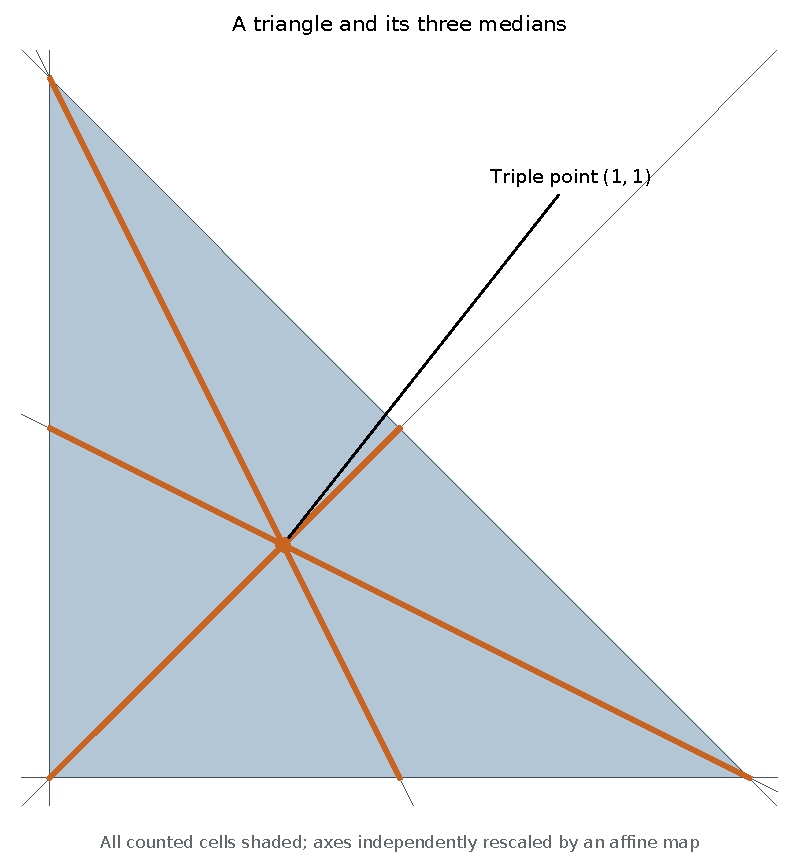
\includegraphics[width=0.75\textwidth]{figures/shared-fan.pdf}
\caption{The exact arrangement~\eqref{upper:median-lines}. Six triangular cells meet around the central triple point, and all six radial sides are shared. This refutes only a literal local incidence reading of the shared-pair statement in Cl\'ement--Bader's Lemma~1; it does not refute their final upper theorem. The figure is newly generated from the integer equations.}
\label{fig:shared-fan}
\end{figure}

The \texttt{SharedFan} module proves the real geometric facts: each designated triangle has nonempty uncut interior, the six interiors are pairwise disjoint, the radial segments are distinct and elementary, and each is a side of two distinct triangles. The proof uses ordinary kernel checking.

This matters when interpreting the Cl\'ement--Bader proof. Its local shared-pair sentence cannot literally bound all shared segments incident to a multiple point by two. An intended assignment of each shared side to one endpoint would be a different assertion requiring global justification. The example has only six triangles, below the reported seven-triangle upper bound at order six; it is therefore not a counterexample to that upper theorem. The present paper leaves that distinction explicit and uses the separate $D_1,D_2$ accounting instead.

Nor can one justify a simple upper bound merely by perturbing every multiple point. For a retained two-triple-point Maiorana $14{:}54$ witness, the four local generic resolution types have triangle counts $52,52,53,52$. These counts were checked with exact arithmetic; they are finite experimental evidence, not a new Lean theorem classifying all perturbations. They demonstrate why a universally nondecreasing smoothing argument needs more than the existence of a small generic perturbation. Our global upper argument never assumes such monotonicity.

\subsection{Formal status and the remaining bridge}

The following division is part of the mathematical claim, not an implementation footnote.
\begin{table}[htbp]
\centering\small
\begin{tabularx}{\textwidth}{@{}lXX@{}}
\toprule
Module or argument & Completed & Still required for a global Lean upper theorem\\
\midrule
\texttt{SharedFan} & Exact real six-line counterexample to the literal local reading. & No general conclusion is inferred from this example.\\
\texttt{FanGeometry} & Uniqueness and propagation of opposite supports; obstruction at opposite rays. & Extract fan strips from arbitrary arrangement cells.\\
\texttt{FanCount} & Cyclic-window double count and $2r-3$ bound. & Supply its geometric selected set.\\
\texttt{CyclicFan} & Actual sector geometry implies the no-long-run property and selected-cardinality bound. & Construct the cyclic sector data globally.\\
\texttt{CleanLineBudget} & Integer consequences of explicitly supplied incidence, charging, and fan inequalities. & Prove those hypotheses for all arrangements in the intended class.\\
Paper-level geometry & Segment identity, clean-line parity charging, and restricted consequences above. & Formal elementary edges, their cell incidences, global summation, and the sharper $d_2\le1$ fan refinement.\\
\bottomrule
\end{tabularx}
\caption{The upper-bound formalization boundary. Every completed module in this table was checked without placeholders; the table does not identify the conditional arithmetic module with a completed geometric upper theorem.}
\label{upper:formal-status}
\end{table}

In particular, \texttt{CleanLineBudget} also contains arithmetic implications with a symbolic parallel-pair term. Those implications do not prove the missing charging lemma with parallels. The nine conditional arithmetic theorems and the geometric fan modules use only the standard axiom set recorded for this development. Exact finite checks on $597$ test arrangements, followed by the imported Maiorana and gallery witnesses, support the accounting and expose implementation mistakes; they do not replace its general proof.

The main unresolved direction is therefore precise. One must control the negatively weighted triple and quadruple points, account for the entire core rather than a chosen subgraph, and separately handle parallel classes. Completing the global Lean extraction would certify the restricted results above. Improving the unrestricted numerical upper envelope requires an additional mathematical idea beyond those formalization tasks.
